\section{Performance analyse}
Tijdens de ontwikkeling van de library is duidelijk geworden dat de performance van de geschreven programma's niet altijd optimaal is. Met name bij programma's die gebruik maken van \emph{timers} en bij programma's met een uitgebreidde grafische boom.

Dit peformance probleem kan twee oorzaken hebben, ten eerste is het mogelijk dat de haskell zijde van de applicatie niet snel genoeg JSON-berichten kan maken en anderzijds is het mogelijk dat Javascript de binnengekomen berichten niet snel genoeg kan verwerken.

Eerst is gekeken naar de peformance van Haskell, hiervoor is voornamelijk gekeken naar de heap omdat het vermoeden was dat Haskell mogelijk te veel geheugen zou gebruiken (mogelijk door een geheugenlek) en voortdurend aan het garbage collecten is. Na een heap profile gemaakt te hebben bleek dat de Haskell code in totaal 600kb aan geheugen gebruikt, en dit getal stabiel is. De Haskell kant gaf dus geen problemen.

De Javascript kant van het project daarentegen geeft een groter probleem. In het ontwerp hebben we ervoor gekozen de grafische boom stateless te maken, als een nieuwe tekenactie door Haskell vertaald wordt, dan krijgt de Javascript kant de hele grafische boom. Het opnieuw  opbouwen van de stage bleek echter kostbaar te zijn en kost Kinetic ongeveer 6 ms (tegen 0.5 ms voor het opnieuw tekenen van dezelfde stage). Om de peformance problemen op te lossen is het daartoe noodzakelijk om incrementele updates te ondersteunen zodat niet steeds de hele stage opnieuw opgebouwt hoeft te worden.

Er is nog wel een optimalisatie uitgevoerd, er was het vermoeden dat er in de Haskell code van Canvas.hs veel peformance verloren zou gaan doordat we \inlinecode{String}s naar \inlinecode{ByteStrings} naar \inlinecode{Text} vertaalde. Het bleek dat de laatste vertaalslag overbodig is, en daartoe is deze verwijderd. Hieronder volgen twee grafieken die het geheugengebruik van de Haskell kant van Canvas.hs demonstreren met en zonder de extra translaties.

Er waren vermoedens dat de oorzaak gevonden kon worden in het omzetten van \inlinecode{Strings} naar \inlinecode{ByteSrings} en vice versa.

\begin{figure}
\begin{center}
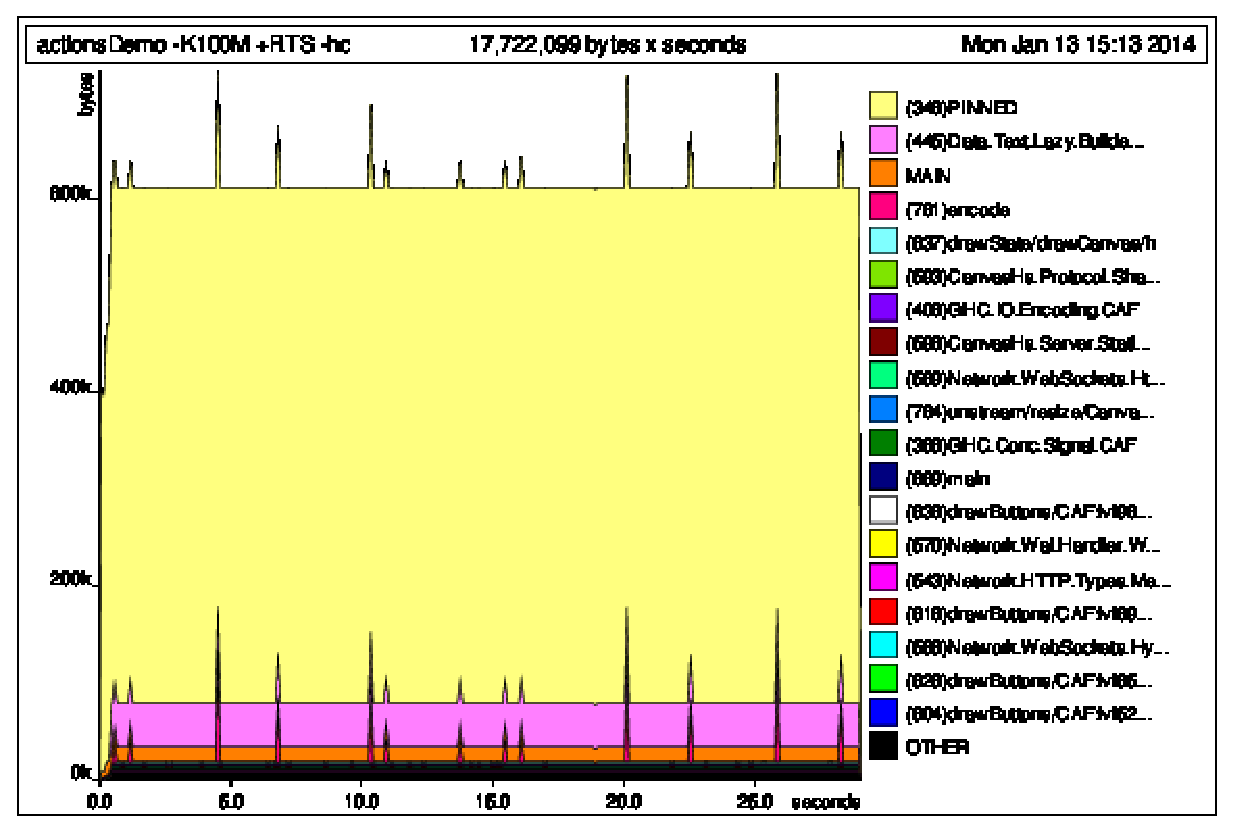
\includegraphics[keepaspectratio,width=0.8\textwidth]{./images/actionsDemoAfterByteStrings.eps}
\caption{Heap profile voor de wijziging}
\label{fig:sub1}
\end{center}
\end{figure}

\begin{figure}
\begin{center}
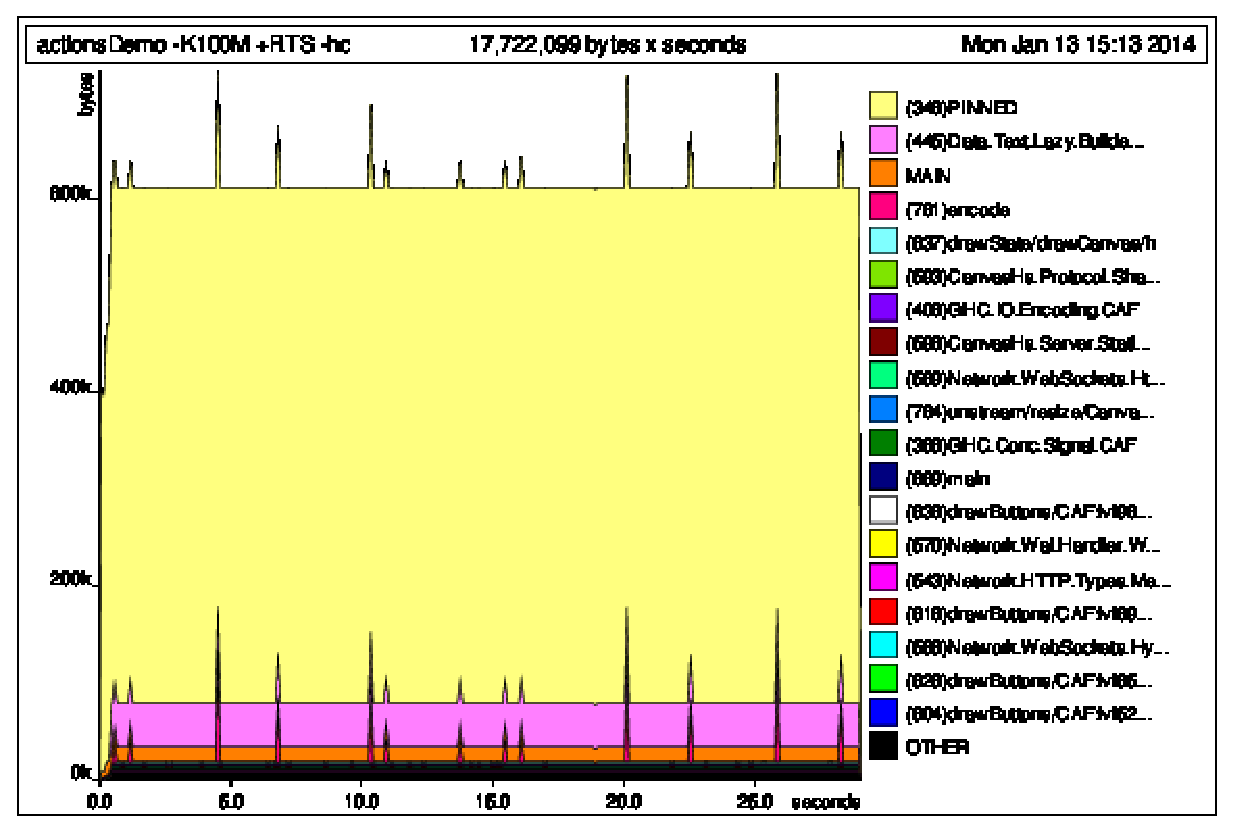
\includegraphics[keepaspectratio,width=0.8\textwidth]{./images/actionsDemoAfterByteStrings.eps}
\caption{Heap profile na de wijziging}
\label{fig:sub1}
\end{center}
\end{figure}

\todo{Schrijven over de wijziging's impact}
